\section{}
% A wooden, simply supported beam of length L is subjected to a uniform load p. Determine the
% beam length and the loading necessary to develop simultaneously σmax = 8.4 MPa and τmax =
% 0.7 MPa. Take thickness t = 0.05 m and depth h = 0.15 m.

A wooden, simply supported beam of length $L$ is subjected to a uniform load $p$. Determine the
beam length and the loading necessary to develop simultaneously $\sigma_{max} = 8.4$ MPa and $\tau_{max} =
0.7$ MPa. Take thickness $t = 0.05$ m and depth $h = 0.15$ m.

\begin{figure}
    \centering
    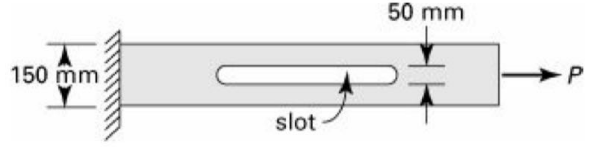
\includegraphics[width=0.35\linewidth]{Questions/Figures/Q5ProblemDiagram.png}
    \caption{Problem diagram for Question 5.}
\end{figure}

Using singularity functions, 
\begin{align*}
    V &= \frac{pL}{2} \langle x - 0 \rangle^{0} - p \langle x - 0 \rangle^{1} \\
    M & = \frac{pL}{2} \langle x - 0 \rangle^{1} - \frac{p}{2} \langle x - 0 \rangle^{2} \\
\end{align*}

By symmetry, the maximum bending moment occurs at the center of the beam. From inspection, the max shear force is at the supports. Then,
\begin{align*}
    V_{\max} &= \frac{pL}{2} \\
    M_{\max} &= \frac{pL^2}{8}
\end{align*}

Moment of inertia,
\begin{align*}
    I_z &= \frac{th^3}{12} = \frac{(0.05)(0.15^3)}{12} = 1.4063\times 10^{-5} \text{ m}^4
\end{align*}

From bending,
\begin{align*}
    \sigma_{\max} &= \frac{M_{\max} y}{I_z} \\
    &= \frac{pL^2 y}{8 I_z} \\
    \implies pL^2 &= \frac{16 I_z \sigma_{\max}}{h} \\
    &= \frac{16 (1.4063\times 10^{-5}) (8.4\times 10^6)}{0.15} \\
    &= 12600 \text{ N}
\end{align*}

From shear on a rectangular cross section,
\begin{align*}
    \tau_{\max} &= \frac{3V_{\max}}{2A} \\
    &= \frac{3pL}{4(0.05)(0.15)} \\
    &= 100pL \\
    \implies pL &= 7000 \text{ N}
\end{align*}

Solving with Matlab,
\begin{lstlisting}[language=Matlab]
syms p L
eqn1 = p*L^2 == 12600;
eqn2 = p*L == 7000;
sol = vpasolve([eqn1, eqn2], [p, L])
\end{lstlisting}

\begin{verbatim}
p: 3888.8888888888888888888888888889
L: 1.8
\end{verbatim}